\subsection{BiLM}
\label{sec:bilm}

In front of the paper, we propose a Word Sense Induction method base on WordNet and pre-train Language Model.
But for more thought, we only extract the paragraph grained representations though it's a similarity to the meaning of the center word.
And we only match the word meaning from WordNet. It has some deviation between actual meaning and WordNet meaning.
For the more, In our method, the rule of division top-N is the decision by practical experience. It somethings don't work well.

For a naive mind, we can change the paragraph grained to the word grained and then clustering word meaning from sample sentences.
It means that we should build a more fine-grained from around word rather than common word embedding, like ELMo~\cite{Peters:2018}, Bert.
But if we directly replace word to context word embedding, It's too much noise in the word embedding spacing between same meaning word.
It causes that direct cluster ELMo embedding vector don't better than other pre-train word embedding.
Refer the Bask's Work~\cite{baskaya2013ai}. We using substitute vectors instead of directing using word embedding producing by ELMo.
It's mean that we choose some word which is the similarity to the meaning of this word in their sentence.
The way of choose substitute word is base on reusing Language Model ELMo.
In addition to that work, we also use a skill to get unequal length similarity meaning substitute word.
The most similarity substitute word will be cluster to several clusters. 

\begin{figure*}[ht]
    \begin{center}
    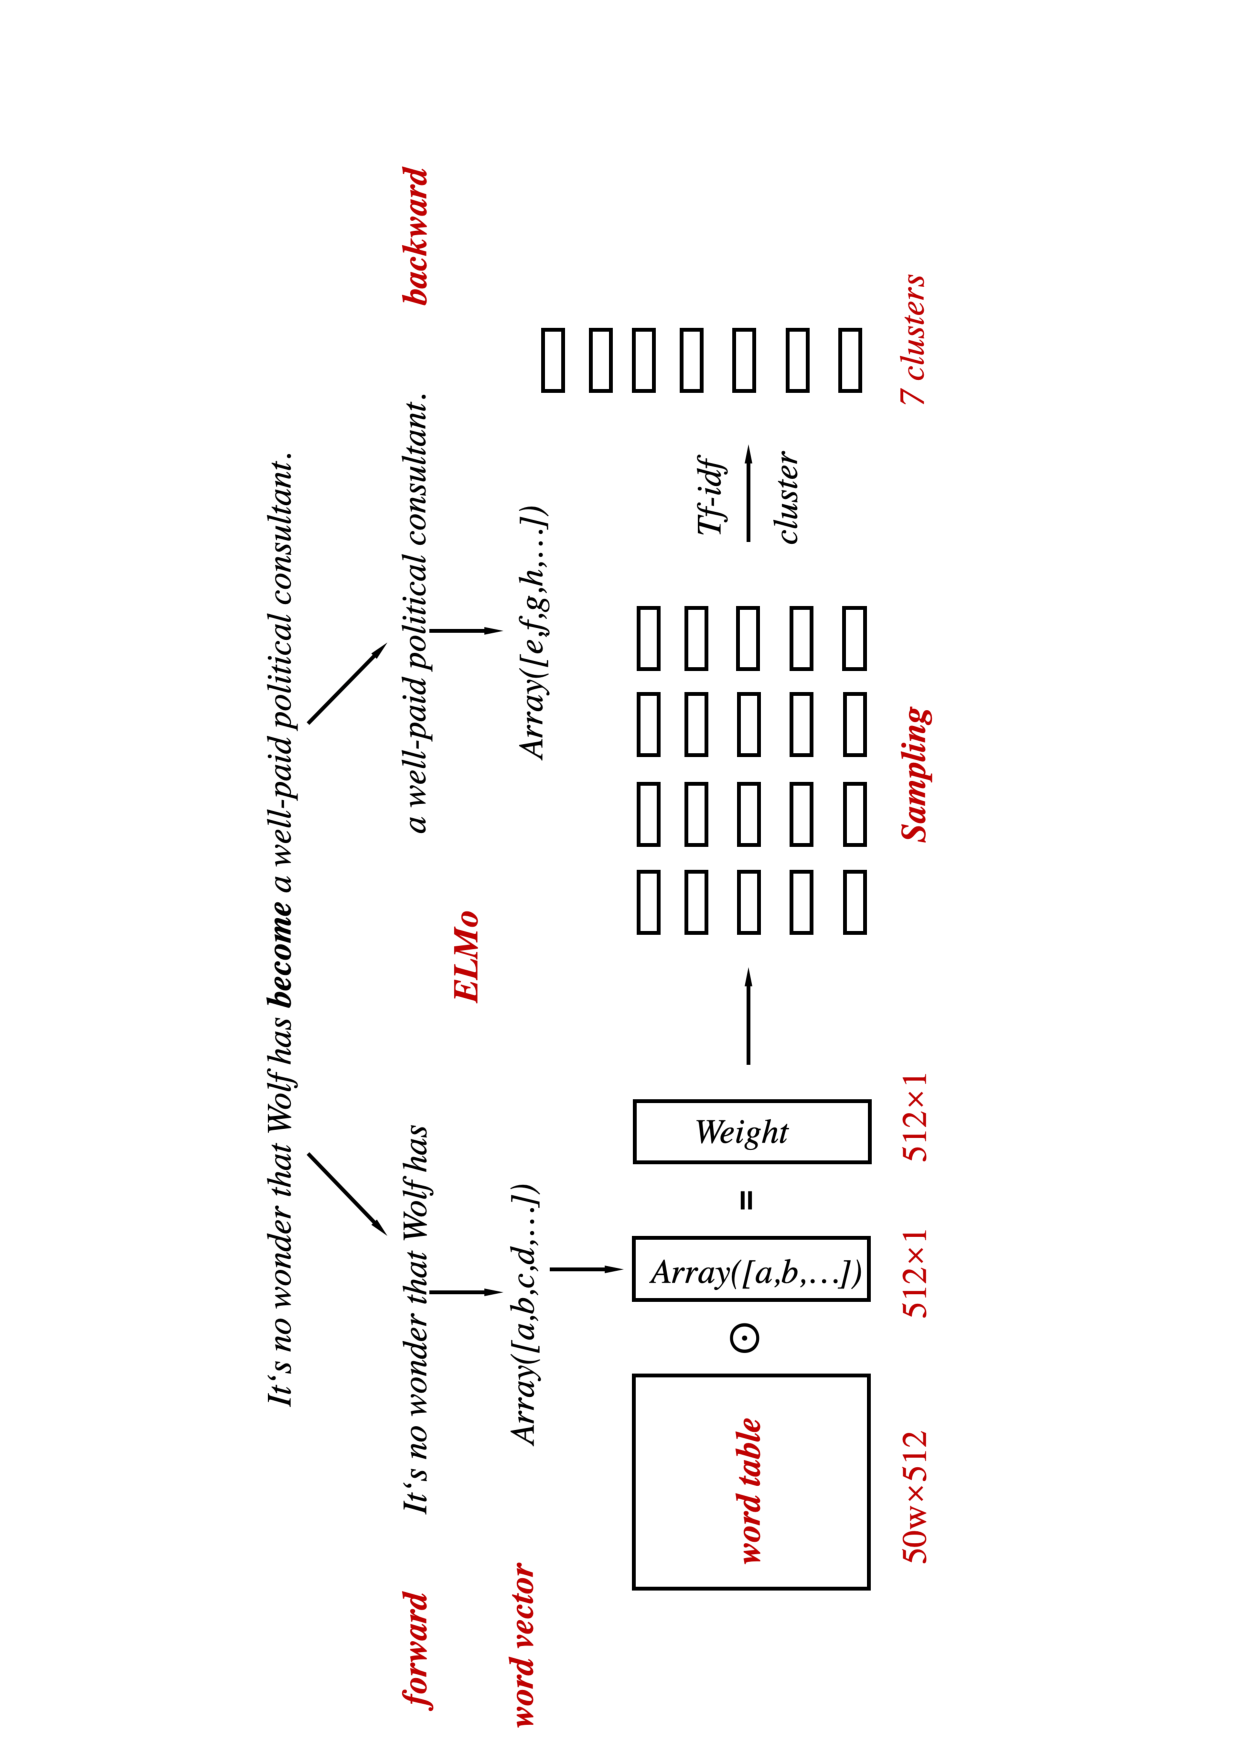
\includegraphics[width=0.85\textwidth]{figures/BiLM.pdf}
    \end{center}
    \caption{The overview of model structure}
    \label{fig:overall_model}
\end{figure*}

\paragraph{Substitute Vectors}
Language Model is an intuitive way we to get the meaning of the word from context word from sample sentence.
But for the most time, directly replace the word by word embedding is meaning amplification cluster distance.
It has low robustness when the word vector causing by Language Model have noise.
So refer to the work of Neural biLM~\cite{amrami-goldberg-2018-word}, we use BiLM to change word vector to a similar word.
This way reduce the word noise meaning, and amplification the important meaning.
And in the actual, We random choose most similarity word base Language Model weight dot local word vector.
By multi choosing, we get the most similarity word no matter what the num of word most similarity.

\paragraph{BiLM \& Cluster embedding}
Language Model is an obvious idea in Word Sense Induction problem.
In the Substitute Word process, we using Language Model for twice.
First, we extract context word meaning to center word vector by forwarding Language Model.
And we random choose the most similarity word from the Matrix of Language model weight dot center word embedding.
It's product by backward Language Model.
It's a process of word vector to the word.
And then we use the substitute word to the cluster, It also needs a word embedding process though It does not have context word.
So In our second method, we multi-use Language Model to extract words actual meaning.

